% Chapter 1

\chapter{Introducción general} % Main chapter title

\label{Chapter1} % For referencing the chapter elsewhere, use \ref{Chapter1} 
\label{IntroGeneral}

%----------------------------------------------------------------------------------------

% Define some commands to keep the formatting separated from the content 
\newcommand{\keyword}[1]{\textbf{#1}}
\newcommand{\tabhead}[1]{\textbf{#1}}
\newcommand{\code}[1]{\texttt{#1}}
\newcommand{\file}[1]{\texttt{\bfseries#1}}
\newcommand{\option}[1]{\texttt{\itshape#1}}
\newcommand{\grados}{$^{\circ}$}

%----------------------------------------------------------------------------------------

Esta sección presenta las motivaciones, alcance y objetivos así como la comparativa de productos similares en el mercado.

%----------------------------------------------------------------------------------------
\section{Motivación}

En muchas zonas del Perú, los pequeños agricultores se ven afectados por los fenómenos ambientales como las sequías y heladas que repercuten directamente en sus cosechas. Por otro lado, constantemente realizan muchas operaciones manuales que podrían automatizarse para generar eficiencias en el uso de los recursos.

Uno de los principales fenómenos que afecta mucho a la producción agrícola son las heladas, normalmente este fenómeno se produce durante las madrugadas dañando toda la cosecha. Una forma eficaz de proteger los sembríos de las heladas es detectar a tiempo el fenómeno y luego rociar abundante agua en la zona.

Es por esa razón que el espíritu de este prototipo es poner al alcance de los pequeños agricultores un sistema de riesgo autónomo que permita automatizar los procesos de riego y tener la capacidad de monitorear las diferentes variables ambientales para tomar una acción correctiva.

%----------------------------------------------------------------------------------------

\section{Alcance y objetivos}

Esta memoria describe el proceso de diseño y fabricación de un prototipo de un sistema de riego autónomo con conectividad inalámbrica que permita controlar dos (4) electroválvulas independientes y una (1) motobomba para mayor presión en el flujo de agua. Asimismo, el sistema estará equipado por sensores de presión atmosférica, temperatura y humedad ambiental.

La información será visible a través de una pantalla LCD y tendrá un joystick de dos ejes para su control. También dispondrá de un \textit{Real Time Clock} (RTC) para contabilizar el tiempo.

Como parte del alcance se ha contemplado lo siguiente:

\begin{enumerate}
	\item Diseño del \textit{hardware} del sistema de riego autónomo.
	\item Diseño de la \textit{PCB}.
	\item Ensamblaje.
	\item Diseño del \textit{firmware} del sistema de riego autónomo basado en el microcontrolador ESP32 o similar.
	\item Diseño de la caja 3D.
	\item Pruebas.
\end{enumerate}

El presente prototipo en esta primera etapa no incluye:
\begin{enumerate}
	\item Diseño e implementación de la arquitectura nube donde estarán alojados la API, aplicación web y servidor MQTT.
	\item Diseño e implementación de la API que se comunicará con la aplicación web o móvil.
	\item Diseño e implementación de la aplicación web o móvil para control remoto de los parámetros.
	\item Actualización del \textit{firmware} del microcontrolador para que soporte la comunicación MQTT con el \textit{broker}.
	\item Diseño e implementación de sensores externos e inalámbricos para monitorear la temperatura y humedad de la tierra.
\end{enumerate}

Para el desarrollo del presente proyecto se supone que:
\begin{enumerate}
\item Se importará de China los siguientes componentes electrónicos:
	\begin{itemize}
	\item Un microcontrolador ESP32 o similar.
	\item Un convertidor USB a TTL UART.
	\item Un chip DS3231 ''\textit{Real Time Clock}'' o similar.
	\item Una pantalla LCD de 2.4'' o 3.5''.
	\item Un sensor de temperatura, humedad y presión atmosférica (BME280) o similar.
	\item Un \textit{joystick} de 2 ejes (x-y).
	\item Otros componentes: resistencias, capacitores, diodos, etc.
	\end{itemize}	
\item Se dispondrá de un mínimo de 704 horas requeridas para realizar el prototipo.
\item Se dispondrá del presupuesto económico para realizar las compras requeridas.
\item Se dispondrá del \textit{software} requerido para el prototipo: IDE del microcontrolador, KiCad 6 y Autodesk Fusion360.
\item Se dispondrá de un proveedor para la elaboración de la PCB.
\item Se dispondrá de un proveedor local para las impresiones 3D de la carcasa.
\end{enumerate}

%----------------------------------------------------------------------------------------
\newpage
\section{Estado del arte}

En la actualidad podemos encontrar diferentes empresas que comercializan programadores de riego o \textit{timers} que cumplen dicha función. Sin embargo en muchos de los casos son dispositivos muy generales y con poca flexibilidad.
\newline
\begin{table}[h]
	\begin{center}
		\begin{tabular}{ p{1cm} p{2cm} p{3cm} p{2cm} p{2cm} }

			\hline 
	 		\textbf{Item} & \textbf{Marca}  & \textbf{Modelo} & \textbf{Precio} & \textbf{Salidas}	\\
			\hline 
			1 & Rain Bird & 1ZEHTMR & S/ 295.00 & 1 salida	\\
			2 & Rain Bird & ESP-RZXe & S/ 480.00  & 8 salidas	\\
			3 & Rain Bird & TM2-6-230 & S/ 658.00  & 6 salidas	\\
			4 & Rain Bird & TM2-12-230 & S/ 1561.00  & 12 salidas	\\
			5 & HUNTER & BTT101 & S/ 300.00  & 1 salida	\\
			6 & GALCON & 80024/8 & S/ 765.00  & 8 salidas	\\
			\hline 
		\end{tabular}
		\caption{Tabla comparativa de fabricantes de programadores de riego o similares}
	\end{center}
\end{table}

\begin{figure}[h]
	\centering
	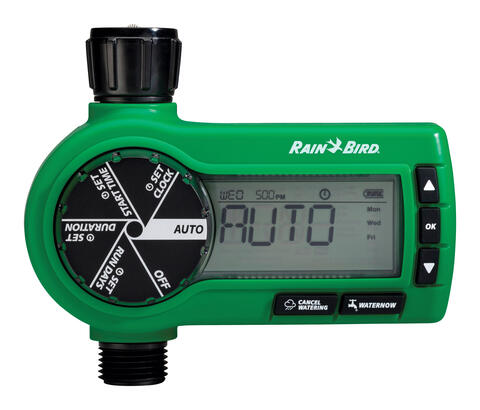
\includegraphics[width=0.4\textwidth]{1ZEHTMR}
	\caption{Rain Bird 1ZEHTMR.}
\end{figure}

\begin{figure}[h]
	\centering
	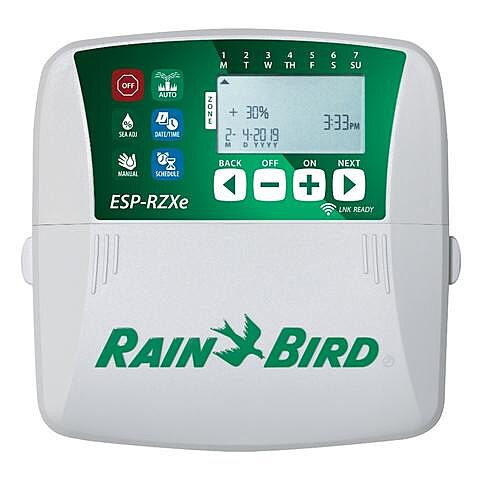
\includegraphics[width=0.4\textwidth]{ESP-RZXe}
	\caption{Rain Bird ESP-RZXe.}
\end{figure}

\begin{figure}[h]
	\centering
	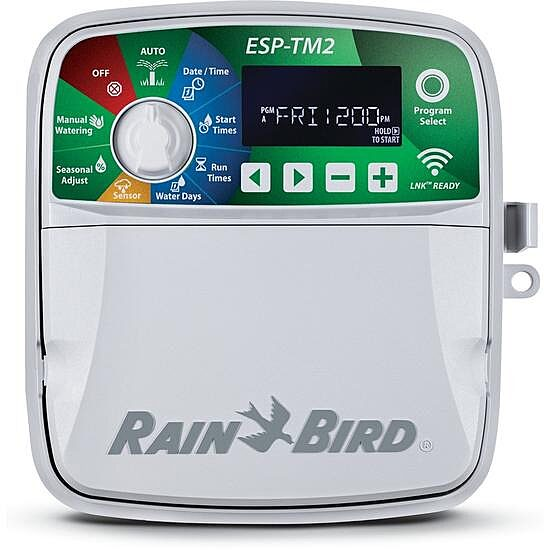
\includegraphics[width=0.4\textwidth]{ESP TM2-X-230}
	\caption{Rain Bird ESP TM2-X-230.}
\end{figure}

\begin{figure}[h]
	\centering
	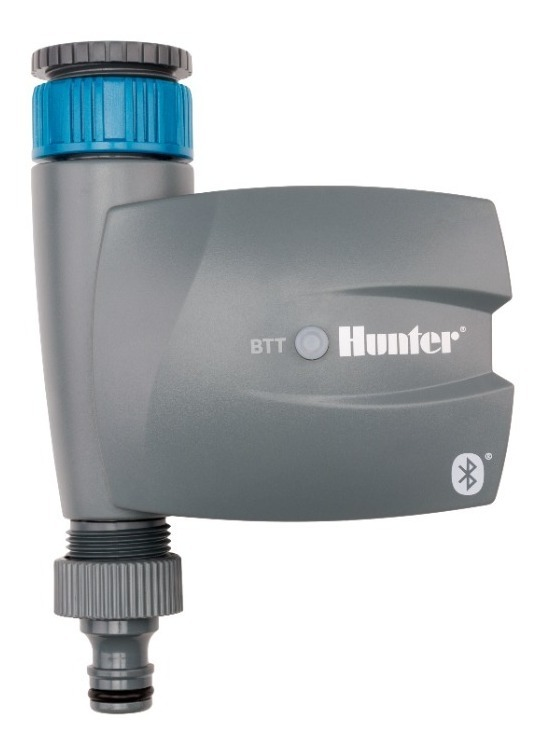
\includegraphics[width=0.4\textwidth]{BTT101}
	\caption{Hunter BTT101.}
\end{figure}

\begin{figure}[h]
	\centering
	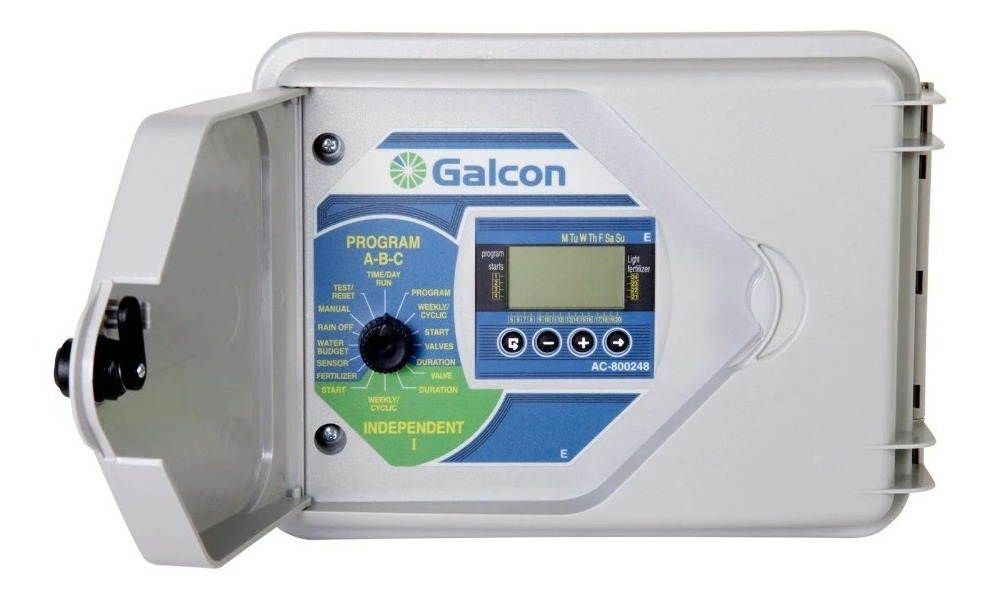
\includegraphics[width=0.4\textwidth]{80024-8}
	\caption{Galcon 80024-8.}
\end{figure}
%----------------------------------------------------------------------------------------
